\chapter{Ausarbeitung}
\section{Aufgabe 1}
\subsection{a}
Float'-Ambiguities $\bm{\hat{a}} = \left[1.03 \quad 1.54\right]$, Kovarianzmatrix $\bm{Q_{\hat{a}}} = \begin{bmatrix}
	5.34 & 3.84 \\
	3.84 & 2.80
\end{bmatrix}$ \\\\
Fixieren mit Einfaches Runden:
\begin{equation*}
	\bm{\check{a}_{er}} = \begin{bmatrix}
		1\\2
	\end{bmatrix}
\end{equation*}
Fixieren mit Bootstrapping
\begin{align*}
	& \bm{\check{a}_{b}}(1) = round(1.03) = 1 \\
	& \bm{\check{a}_{b}}(2) = round(1.54 - \frac{3.84}{5.34}(1 - 1.03)) = 2
\end{align*}
Beides mal kommen zum gleichen Ergebnis bei dem Fall.
\subsection{b}
\begin{equation*}
	\bm{Z}_1 = \begin{bmatrix}
		-1 & 1 \\
		1 & 0
	\end{bmatrix} ,\qquad \bm{Z}_2 = \begin{bmatrix}
	3 & 1 \\
	1 & 0
\end{bmatrix}
\end{equation*}
\begin{equation*}
	\bm{Z} = \bm{Z}_2 \cdot \bm{Z}_1 = \begin{bmatrix}
		2 & -3 \\
		-1 & 1
	\end{bmatrix}
\end{equation*}
Kovarianzmatrix nach der Transformation:
\begin{equation*}
	\bm{Q}_z = \bm{Z} \cdot \bm{Q_{\hat{a}}} \cdot \bm{Z}' = \begin{bmatrix}
		0.48 & -0.12\\
		-0.12 & 0.46
	\end{bmatrix}
\end{equation*}
Die Korrelationskoeffizienten:
\begin{gather*}
	r_1 = \frac{3.84}{\sqrt{5.34 \cdot 2.80}} = 0.993 \\
	r_2 = \frac{-0.12}{\sqrt{0.48 \cdot 0.46}} = -0.255
\end{gather*}
Die Korrelationskoeffizienten hat sich deutlich verringert.\\\\
Danach wird $\bm{\check{z}}$ jeweils mit einfachen Funden und Bootstrapping fixiert.
\begin{gather*}
	\bm{z} = \bm{Z} \cdot \bm{\hat{a}} = \begin{bmatrix}
		2.56 \\
		0.51
	\end{bmatrix}\\
	\bm{\check{z}}_{er} = \begin{bmatrix}
		3 \\ 1
	\end{bmatrix} \\
	\bm{\check{z}}_{b} = \begin{bmatrix}
		3 \\ 1
	\end{bmatrix}
\end{gather*}
beide Ergebnisse führen: $\bm{\check{a}} = \begin{bmatrix}
	0 \\ 1
\end{bmatrix}$, Dieses Verfahren ändert den Bereich in dem die Integer Werte gesucht werden. Der Bereich ist größer als der des einfachen Rundens bzw. in (a).
\subsection{c}
Der Beweis kann mit vollständiger Induktion durchgeführt werden.
\begin{gather*}
	\bm{Z}_1 = \begin{bmatrix}
		z_1 & 1 \\
		1 & 0
	\end{bmatrix}\\
\det(\bm{Z}_1) = -1
\end{gather*}
jetzt muss man beweisen, für jede $\bm{Z}(i) = \begin{bmatrix}
	z & 1\\
	1 & 0
\end{bmatrix} \cdot \begin{bmatrix}
a & b \\
c & d
\end{bmatrix}$, gilt $\det(\bm{Z}) = \pm 1$, wobei $\bm{Z}(i-1) = \begin{bmatrix}
a & b\\
c & d
\end{bmatrix}$
\begin{gather*}
	\bm{Z}(i) = \begin{bmatrix}
		az + c & bz + d \\
		a & b
	\end{bmatrix} \\
\det(\bm{Z}(i)) = abz + bc - abz - ad = bc - ad = -\det(\bm{Z}(i-1))
\end{gather*}
Deswegen ist $\det(\bm{Z}(i)) = (-1)^{i}$\\\\
$\bm{Z}$ aus Abschnitt b ist eine ganzzahlige unimodulare Matrix.
\clearpage

\section{Aufgabe 2}
\subsection{a}
Nachdem Ausführung der verschiedenen Verfahren kriegt man gleiche Ergebnisse.
\subsection{b}
SQNORM aus Methode 2:
\begin{equation*}
	SQNORM = \begin{bmatrix}
		1.95 \\
		28.77
	\end{bmatrix}
\end{equation*}
Testwert $T = \tfrac{1.95}{28.77} = 0.0678 < 0.5$, der Test schreitet den Schwellenwert nicht über.

\section{Aufgabe 3}
Matlan Version: R2021a \\
AMD Ryzen 5 3600X 6 Core Processor 3.80 GHz, RAM 16GB\\\\
Die Beziehung zwischen Rechenzeit und Vektorgröße:
\begin{figure}[htbp]
	\centering
	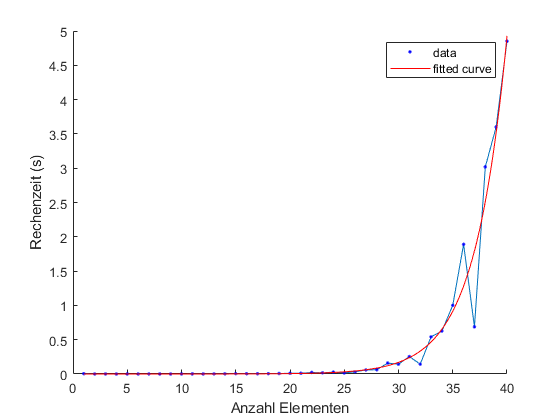
\includegraphics[width=0.7\textwidth]{images/A3} 
	\caption{Aufgabe3} 
	\label{fig:A3}
\end{figure}\\
Die Rechenzeit hat sich schnell vergrößert mit dem Zustieg der Elementenanzahl. Deswegen wird die Daten mit einer Exponentialfunktion approximiert. 


